\documentclass{article}
\usepackage[utf8]{inputenc}
\usepackage{graphicx}

\title{6.036 project 2}
\author{Rebecca Corcillo }
\date{April 2014}

\begin{document}

\maketitle

\section{}
In the M-step, we need to re-estimate the parameters based on the word-tag counts.  We have real tag-counts taken from labeled data as well as expected counts based on the current model in the E-step, for each of the four theta categories.  These tag-counts are passed into our M-step function and our goal was to find the normalized parameter estimates.  \newline
The count for a tag t is based on the formula $n(t) = c * r(t) + e(t)$ where c is the weight assigned to the real counts (assigned as 100 in the code), $r(t)$ is the real tag count and $e(t)$ is the estimated tag count.  We needed to find these counts of tags and normalize them to get the probability of each tag occuring.  For the simplest case of pt, which is just a column vector, we simply need to divide the number of times a certain tag occurs (from nt) by the total number of tags to get the probabilty that this tag occurs, like so: 
\begin{verbatim}
        pt = c*t + et  #this is actually nt right now, will normalize
        for num in pt:
            num/=np.sum(pt)
\end{verbatim}
Ptw is a TxW matrix giving the probabilities of a jth word given an ith tag and ntw is a TxW matrix giving the number of times a jth word occurs given an ith tag. To calculate a specific $p(w|t)$ , the probability of a word given a tag, we must find $n(w|t)$, the number of words w that occur given a tag, and normalize this number by dividing by the total number of words given that tag (which is the sum of the tags row).  Even though ptpw and ptnw represent the probability of a word j given it preceds a tag i and the probability of a word j given it follows a tag i, respectively, the calculations are the same as ptw, using their respective expected number and real number matrices. Here is the code for ptw, ptpw and ptnw:

\begin{verbatim}
        ptw= c*tw + etw  #words given its tag
        for row in ptw:
            for col in row:
                col/=np.sum(row)
             
        ptpw = c*tpw + etpw  #words given preceding tag 
        for row in ptpw:
            for col in row:
                col/=np.sum(row)
             
            
        ptnw = c* tnw + etnw  #words given following tags
        for row in ptnw:
            for col in row:
                col/=np.sum(row)
\end{verbatim}

\section{}
We have an overall list of names of tags called T.  We have an overall list $p(t)$ that has the probabilities of each of the tags at the corresponding index.  Ptw is a matrix where the rows correspond to the tags in T at the same index, columns correspond to the word at the same index in our dictionary W, and the intersection of a row and column i and j represents the probability of word at index j given the tag at index i.  \newline To get the posterior from model A, we must find the joint distribution of a given word and a given tag, making an intermediate vector of joint probabilities of a given  word and all of the tags.  To get the posterior probability, we divide the joint probability vector by the sum of all entries in the joint probability vector (this sum is the probability of the given word). We continuously contruct etw by adding the probability vector to the column of etw corresponding to the word's position in the dictionary. I did this with the following code:
\begin{verbatim}
	for sent in wordList: #sentence is a row vector
	   for pos in range(len(sent)): #index of word in sentence vecto    
	       jointProbVector = pt*ptw[:,sent[pos]]
	       pw = np.sum(jointProbVector)
	       posteriorProb = jointProbVector/pw		
	       etw[:,sent[pos]]+=posteriorProb
	et=np.sum(etw, axis=1)		
        return et, etw, etpw, etnw
\end{verbatim}
In model B, our work is very similar to what we do in model A, except we must now include the probability of the previous word given the current tag in the calculation of posterior probablity.  We must also account for edge conditions due to the fact that the first word does not have a word preceding it.  The probability of the first word is calculated based only on itself and its tag, like the posterior probabilities were in model A. When we calculate etw, we do so in the same way as part A, adding to the column of etw corresponding to the word's position in the dictionary whose posterior probability we just calculated.  When we calculate etpw, we do something very similar but instead change the column corresponding to the position-1 of the word whose posterior probability we just calculated. We calculate et the same way as we did in model A, by making each entry in the vector the sum of the corresponding row in etw.

\begin{verbatim}     
   	for sent in wordList: #sentence is a row vector
	   for pos in range(len(sent)): #index of word in sentence vector   
                if pos==0:
                    jointProbVector = pt*ptw[:,sent[pos]] 
                else:
                    jointProbVector = pt*ptw[:,sent[pos]]*ptpw[:,sent[pos-1]]                
                pw = np.sum(jointProbVector)
                posteriorProb = jointProbVector/pw
                
                etw[:,sent[pos]]+=posteriorProb
                etpw[:,sent[pos-1]]+=posteriorProb

	et=np.sum(etw, axis=1)	
	return et, etw, etpw, etnw
\end{verbatim}

Again, model C works in a very similar way to model B. Instead of just inspecting the word before a given tagged word, we must also inspect a word after the given word.  We now need four if conditions:  If the length of the sentence is 1, we do as we did in part a, if the position of the word is 0, we only look at the next word and the current words probabilities, if the word's position is that of the last word in the list, we only look at that words probability and the probability of the word before it, and finally, if none of these are met, we look at the previous word, the current word and the future word.  All this can be seen in the following code:  \begin{verbatim}
for sent in wordList: #sentence is a row vector
        for pos in range(len(sent)): #index of word in sentence vector   
            if len(sent)==1:
               jointProbVector = pt*ptw[:,sent[pos]]                                         
            elif pos==0:
                jointProbVector = pt*ptw[:,sent[pos]]*ptnw[:,sent[pos+1]]    
            elif pos==len(sent)-1:
           	jointProbVector=pt*ptw[:,sent[pos]]*ptpw[:,sent[pos-1]] 
            else:
                jointProbVector = pt*ptw[:,sent[pos]]*ptnw[:,sent[pos+1]]**ptpw[:,sent[pos-1]]
            
            pw = np.sum(jointProbVector)
            posteriorProb = jointProbVector/pw
            
            etw[:,sent[pos]]+=posteriorProb
            etpw[:,sent[pos-1]]+=posteriorProb
            etnw[:,sent[pos+1]]+=posteriorProb
                        
    et=np.sum(etw, axis=1)	
    return et, etw, etpw, etnw 
\end{verbatim} 
\section{}
To make predictions, we will look at pt, ptw, ptpw and ptnw, depending on the given model letter.  Whatever the model number, we are trying to see which tag has the highest probability of being assigned to a specific word and that will allow us to predict what the label of that word will likely be.  Given a test sentence, we will use each model of tagging on that sentence use it to predict the labels of each word in the sentence.  We basically had to make this matrix of joint probabilities and find the max tag probability for each word.  For mixture model A, we make the jointProbabilityVector by $pt*ptw[:,sent[pos]]$ and then find the index of the largest entry of the matrix, which will correspond to the most likely tag for the given word we were looking at in the sentence.  We add this tag label to our current prediction list, which will, at the end of the for loop iterating through words in a given sentence, contain a prediction for each word in the sentence we were on.  We add this list to the overall pred list and repeat on each sentence in the word list.  Predict A was done with the following code: 
\begin{verbatim}
	pred = []
	for sent in wordList: #for sentence in sentences
		cur_pred = []
		for pos in range(len(sent)): #for word in sentence
			jointProbVector = pt*ptw[:,sent[pos]]                                         
            pred_tag = np.argmax(jointProbVector) #gets max tag for given word
			cur_pred.append(pred_tag)
		pred.append(cur_pred)
	return pred\end{verbatim}

For predict B, we do something very similar to predict B, the only difference is in how we construct our jointProbabilityVector.  If we're at the first position, it is an edge case and we can only look at the current word.  Otherwise, we can calculate the joint probability vector using both the current word and the word before it. 
\begin{verbatim}
	for sent in wordList:
		cur_pred = []
		for pos in range(len(sent)):
            if pos==0:
                jointProbVector = pt*ptw[:,sent[pos]]
            else:
                jointProbVector = pt*ptw[:,sent[pos]]*ptpw[:,sent[pos-1]]
                        
            pred_tag = np.argmax(jointProbVector)
			cur_pred.append(pred_tag)
		pred.append(cur_pred)

	return pred \end{verbatim}
Finally, to do C, we just calculate the jointProbabilityVector using the formula for model C.  We have to keep in mind the edge conditions of if the word length is 1, if the word's position is 0, or if the word is the last word and adjust our jointProbabilityVectors accordingly.  Again, we take the index of the largest value in the jointProbabilityVector to be the index of the predicted tag for that word.  We accomplish this with the following code. \begin{verbatim}	for sent in wordList:
		cur_pred = []
		pos = 0
		for pos in range(len(sent)):
            if len(sent)==1:
                jointProbVector = pt*ptw[:,sent[pos]]
            elif pos==0:
                jointProbVector = pt*ptw[:,sent[pos]]*ptnw[:,sent[pos+1]]
            elif pos==len(sent)-1:
                jointProbVector = pt*ptw[:,sent[pos]]*ptpw[:,sent[pos-1]]
            else:
                jointProbVector = pt*ptw[:,sent[pos]]*ptpw[:,sent[pos-1]]*ptnw[:,sent[pos+1]]
			pred_tag = np.argmax(jointProbVector)
            cur_pred.append(pred_tag)
		pred.append(cur_pred)
	return pred \end{verbatim}

\section{}
(a) In this case, there is only training data and no testing data, which means we are just training the three models classifiers with all the training data. We evaluate the tagging accuracy on the test sentences by calling on task1(), which will tell us the tagging accuracy for each mixture model.  We see that the tagging accuracy of model A is around 89 percent and the accuracies continue to increase in model B and then again in C.  \newline 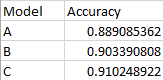
\includegraphics[width=90mm]{task1A.png} \newline
(b) After calling task2(), our data is half labeled, half unlabeled and the EM iterations will alter the model as the parameters are altered to find the best clusters of word combinations for each tag.  This, in turn, changes the accuracy.  This change in accuracy works as a function of EM iterations; the accuracy generally goes up with more iterations, but may, in some cases, go down. The accuracy of model A does not change, and stays at around 89 percent.  The accuracy of B and C both increase as a trend with more iterations. The accuracies of this are slightly lower than that of part a, because the algorithm is running with less known labels to train. \newline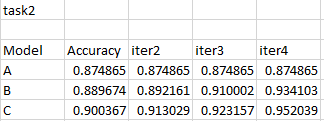
\includegraphics[width=90mm]{task2A.png}\newline



(c) Finally, we call task3() which splits the training data into 1 percent labeled and 99 percent unlabeled. Compared to the test accuracy of the other two scenarios, and to the test accuracy of the model based on the labeled data alone, we see that model A again stays the same with more iterations while model B and C both increase. Here is a table of task3() and its four iterations\newline 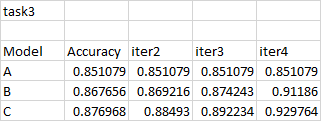
\includegraphics[width=90mm]{task3A.png} \newline

\section{The code you wrote to solve this problem, a description of how you went about it, and
the results of both queries.}
(a) The word with the highest unconditional probability of directly specifying a tag is the comma $(",")$. This means that, without any information about its neighboring words, this word most clearly specifies a tag. The probability with which it specifies a tag is 80 percent. \newline

(b) The metric I designed for determining which word contains the least information about its tag, ignoring the tags surrounding it, worked by finding the word with the least difference between max and min.  Having the least difference between the max and min would mean that the word has the most equally spread distribution between probabilities of tags.
The word that maximizes this metric is bet, likely because it can be used in so many different parts of speech. 

\end{document}